\section{Wrapping}
\label{sec:wrapping}

During the research phase of the project the investigated solutions were
primarily focused on ``wrapping'' an incomplete program such that it becomes a
valid program as a whole, as the OpenJDK team has done for JShell (see
\cref{ssec:a-execution-model-repl}). A solution using templates for various
language constructs was proposed to keep this approach generic across all
languages supported by Spoofax. \Cref{fig:wrapping} shows a diagram which
describes this idea. The diagram shows the wrapping of both the environment
definitions and the incomplete program AST. The environment definitions, in
this case, refer to the language-specific constructs such as class definitions,
function definitions and variable declarations.

\begin{figure}[b]
  \centering
  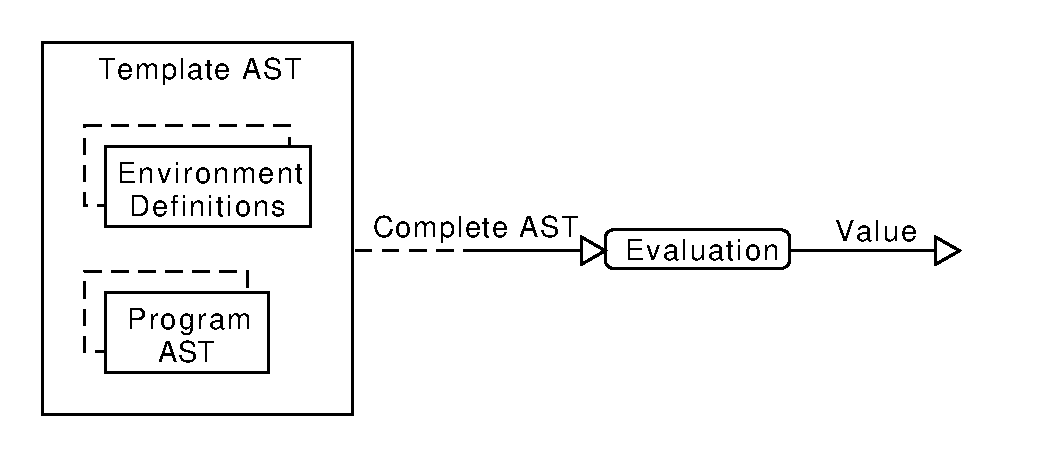
\includegraphics[width=0.5\textwidth]{wrapping}
  \caption{Wrapping the environment definitions and an incomplete program AST
    inside of a template to form a complete and valid program AST.}
  \label{fig:wrapping}
\end{figure}

However, as the project developed and the entry point to DynSem was refactored
significantly (see \cref{sec:dynsem-refactor}), wrapping turned out to be an
unnecessary and inadequate solution for two reasons. Firstly, the ability to
invoke a rule corresponding to any AST, both complete and incomplete,
automatically allows for evaluating incomplete programs without wrapping them
first to form a complete program. Secondly, due to the ability to pass the
semantic components as arguments to a reduction rule, the need of wrapping the
environment definitions (such as functions and variables) became unnecessary
too.

The custom start symbol as described in \cref{sec:esv-extensions} together with
the REPL-specific rules used to obtain and pass execution contexts to DynSem
then already results in a fully functional REPL, without the need to wrap
partial programs inside predefined templates.

%%% Local Variables:
%%% mode: latex
%%% TeX-master: "../main"
%%% End:
